\documentclass[UTF8,a4paper]{ctexart}%设置a4纸和中文
\ctexset{section/format=\Large\bfseries}%设置标题左对齐
\usepackage{amsmath} % 使用align
\usepackage[margin=1in]{geometry}%设置A4值的边界
\usepackage{graphicx}%插入图片
\author{qhy}%作者
\date{\today}%日期
\title{计算机组成}%标题
\pagestyle{empty}%不显示页码
\begin{document}
  \maketitle
  \tableofcontents
  \newpage
  \section{虚拟存储器}
      \subsection{基本概念}
          \begin{itemize}
            \item 虚拟存储器

            指一个容量非常大的存储器的逻辑模型,借助于磁盘等辅助来扩大主存容量,是指"主存-外存"这一存储层次。

            \item 基本特征

            虚拟空间大于实存空间,虚拟空间由辅存支持。

            \item 虚拟存储器和Cache的比较
                \begin{itemize}
                  \item Cache和主存交换数据的频率比较高,而虚存和主存交换数据的频率比较低。

                  \item Cache是提高存储系统的访问速度,它的所有功能由硬件实现。虚存解决的是存储系统的容量,它的所有功能是由操作系统通过软件和硬件来实现的。

                  \item Cache块的大小是固定的,每块的内容也比较小。虚存每次交换的量比较大。
                \end{itemize}
            \item 三级存储体系(见图\ref{fig1})
                \begin{figure}[!htp]
                  \centering
                  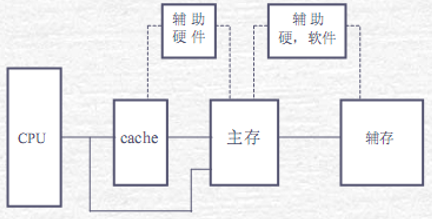
\includegraphics[scale=0.8]{assets/jisuanjizucheng2_14007.png}
                  \caption{三级存储体系}
                  \label{fig1}
                \end{figure}

                在三级存储体系中,\emph{Cache-主存}和\emph{主存-辅存}这两个存储层次的相同点:
                \begin{itemize}
                  \item 出发点相同

                      两者都是为了提高存储系统的性能价格比而构造的层次存储体系,都力图使存储系统的性能接近高速存储器,而价格接近低速存储器

                  \item 原理相同

                      都是利用程序运行时的局部性原理,把最近常用的信息快从相对慢速而大容量的存储器中调入相对高度而小容量的存储器中。
                \end{itemize}

                两者的不同点:
                \begin{itemize}
                  \item 目的不同

                      Cache主要解决主存与CPU的速度差异问题,而虚存就性能价格比的提高而言,主要解决存储容量的问题(另外还包括存储管理、主存分配和存储保护等方面)

                  \item 数据通路不同

                      CPU与Cache和主存之间均由直接访问的通路,Cache不命中时可直接访问主存,而虚存的辅存与CPU之间不存在直接的数据通路,当主存不命中时,只能通过调页解决,CPU最终还是要访问主存。

                  \item 透明性不同

                      Cache的管理完全由硬件完成,对系统程序和应用程序均透明,而虚存管理由软件(操作系统)和硬件共同完成,对系统程序不透明,对应用程序透明(段氏和段页式管理对应用程序"半透明")

                  \item 未命中时的损失不同

                      由于主存的存取时间是Cache的5~10倍,而辅存的存取时间通常是主存的存取时间的上千倍,故虚存未命中时系统的性能损失远大于Cache未命中时的损失。
                \end{itemize}

            \item 几个术语
                \begin{itemize}
                  \item 逻辑地址(虚地址):虚拟程序所提供的地址(是程序的逻辑地址)。

                  \item 虚拟地址空间:程序的逻辑地址空间。

                  \item 物理地址(实地址):CPU用于访问主存的地址。

                  \item 物理地址空间:物理地址所包含的存储空间。

                  \item 程序的再定位:程序进行虚地址到实地址的转换过程。
                \end{itemize}
          \end{itemize}
      \subsection{管理方式}
          \begin{itemize}
            \item 段式管理(见图\ref{fig2})
                \begin{figure}[!htp]
                  \centering
                  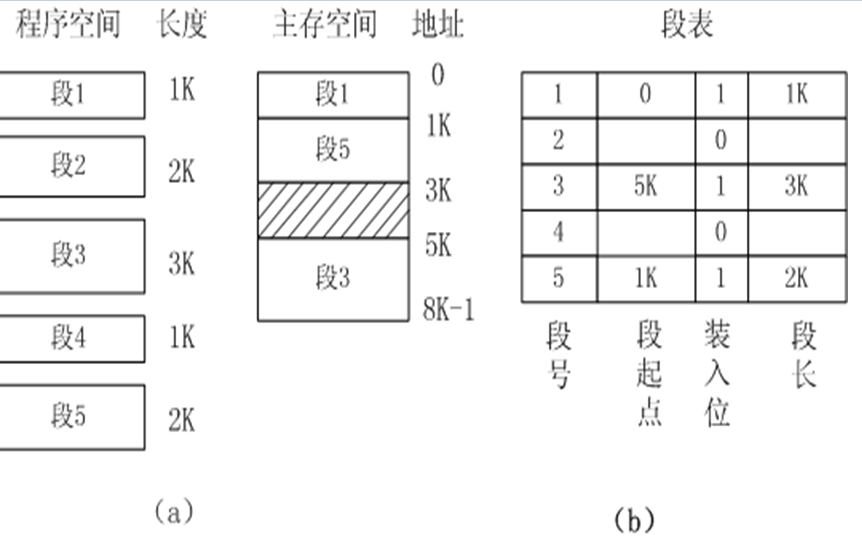
\includegraphics[scale=0.3]{assets/jisuanjizucheng2_9e284.png}
                  \caption{段式管理}
                  \label{fig2}
                \end{figure}

                程序按逻辑结构分段,主存按段来分配存储管理方式。
                程序按逻辑结构分段。
                每一段的长度可以不一样,可以装入主存中的任意位置。
                使用段表来描述程序段在主存空间的位置。

                优缺点:
                \begin{itemize}
                  \item 优点

                      \begin{itemize}
                        \item 段的分界与程序的自然分界相对应
                        \item 段的逻辑独立性使得它易于编译、管理、修改和保护,也便于多道程序共享。
                        \item 某些类型的段(堆栈,队列)具有动态可变长度,允许自由调度以便有效利用空间。

                      \end{itemize}

                  \item 缺点

                      段间的零碎空间(碎片)不好利用。

                \end{itemize}

            \item 页式管理(见图\ref{fig3})
                \begin{figure}[!htp]
                  \centering
                  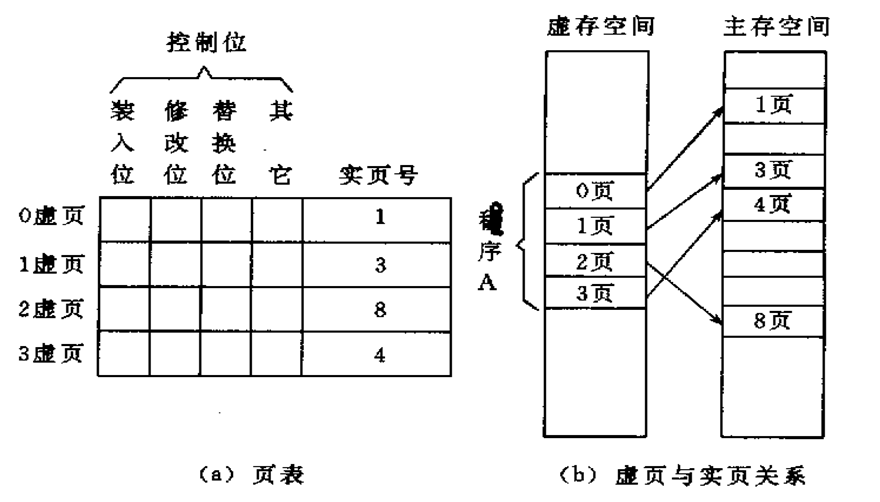
\includegraphics[scale=0.3]{assets/jisuanjizucheng2_5f756.png}
                  \caption{段式管理}
                  \label{fig3}
                \end{figure}

                辅存和主存空间分为页,主存按页来分配的管理方式。
                每一页的大小是相同的。
                \begin{itemize}
                  \item 优点
                      \begin{itemize}
                        \item 造页表方便
                        \item 新页调入容易
                        \item 主存空间利用率高
                      \end{itemize}
                  \item 缺点

                      程序的处理,保护和共享不方便。
                \end{itemize}

            \item 段页式管理

                程序分段:段内分页的管理方式。
                也就是前面两种方式的结合。

                虚实地址的变换过程:
                \begin{itemize}
                  \item [1] 形成访问段表项地址
                  \item [2] 将段表项的页表首地址与段内虚页号相加,形成访问页表项的地址
                  \item[3] 将页表项(装入位为1)的实业号和虚地址的页内地址拼接形成访问实存地址。
                \end{itemize}

                优缺点:
                \begin{itemize}
                  \item 优点:兼有段式和页式管理方式的优点。
                  \item 地址变换过程需要多次查表,速度慢。
                \end{itemize}
          \end{itemize}
      \subsection{工作过程}
          \subsubsection*{使用快表加快虚、实地址变换}

              用高速小容量的相联存储器存放最"活跃页"的地址,加快查表过程。

              快表(转换后援缓冲器 TLB):
              由于页表通常在内存中,因而即使逻辑页已经在主存中,也至少要访问两次物理存储器才能实现一次访存,这将是虚拟存储器的存取时间加倍。为了避免对主存访问次数的增多,可以对页表本身实行二级缓存,把页表中最活跃的部分存放在高速存储器中,组成快表。这个专用页表缓存的高速存储部件通常称为\emph{转换后援缓冲器 TLB}。保存在主存中的完整页表称为慢表。

          \subsubsection*{虚拟存储器的工作过程}
              工作过程(见\ref{fig4}):
              \begin{itemize}
                \item [1] 根据用户号、虚页号同时查询页内表和快表。
                \item [2] 若快表不命中而页内表命中,则页可以得到实页地址
                \item [3] 都不命中 ,则查询外页表得到该页的辅存地址。
                \item [4] 按辅存地址将所缺页装入主存,并更换内页表和快表的内容。
              \end{itemize}


              \begin{figure}[!htp]
                \centering
                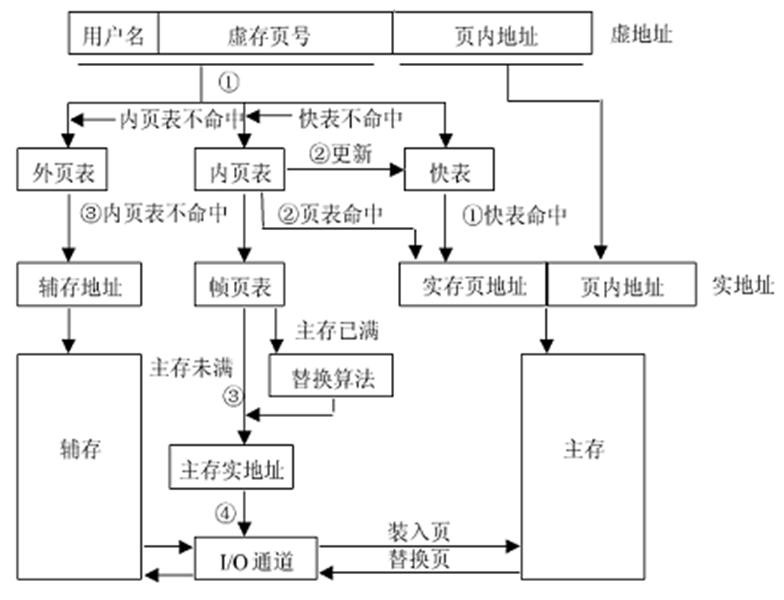
\includegraphics[scale=0.3]{assets/jisuanjizucheng2_94b04.png}
                \caption{页式虚拟存储器工作示意图}
                \label{fig4}
              \end{figure}

              帧页表:用以记录当前主存使用的情况。(主存实业号,占用位,程序号,虚页号,其他)

              外页表:用以登记程序虚页号与辅存地址的对应关系。(虚页号,辅存地址[柱面号,盘面号,扇区号],装入位)

          \subsection{常用的页面替换算法}
              \begin{itemize}
                \item 先进先出算法(FIFO)

                    又称轮转法(RR),先进入内存的页面先替换
                    优点:实现简单
                    缺点:常用的也会被淘汰

                \item 循环检测法

                    让循环多的页面留在主存,记录对页面的访问时间间隔,淘汰时间间隔大的页面。

                    优点:适合循环多的大程序
                    缺点:费时、费空间。

                \item 最近最少使用页面先淘汰(LRU)

                    淘汰最近一段时间最久没有访问的页面。系统开销小。

                \item 最不经常使用的页面先淘汰(LFU)

                    淘汰最近一段时间访问次数最少的页面,对每一页设访问计数器。

                \item 最近没有使用页面先淘汰(NUR)

                    设访问位,选访问位为0的页面进行淘汰。

                \item 最优替换算法(OPT)

                    是理想算法,系统预测作业将要访问的页面,替换预测不被访问或长时间后才被访问的页面。

                \item 随机数替换页面算法

                    无法确定哪些被访问页是最可能不使用时,随机替换一页。
              \end{itemize}

\end{document}
